\chapter{Green Chemistry and Industrial Processes}\label{ch:b3:green-industrial}

Ibuprofen used to be made in six steps that threw away more mass than they
kept: aluminium salts, sodium chloride, ethanol, ammonia and acetic acid left
the plant for every kilogram of drug. Since 1992 a three-step catalytic route
has turned most of the atoms it uses into the product, and its only
by-product, acetic acid, is recovered and sold. This chapter puts numbers on
such comparisons: \omterm{def:b3:green-industrial:atom-economy}{atom economy}, \omterm{def:b3:green-industrial:e-factor}{E-factors} and \omterm{def:b3:green-industrial:pmi}{process mass intensity}; it then
looks at solvents, energy and \omterm{def:b3:green-industrial:lca}{life-cycle assessment}, at how some of the largest
chemical processes were made cleaner, and at what \omterm{def:b3:green-industrial:feedstock}{renewable feedstocks} and
\omterm{def:b3:complex-kinetics:enzyme}{enzymes} change.

\begin{recall}
The school volume introduced \omterm{def:b3:green-industrial:atom-economy}{atom economy} and \omterm{def:b3:green-industrial:green-chemistry}{green chemistry}; the Year 1
volume yields; the Year 2 volume reactors, conversion, selectivity, residence
time, single-pass conversion, recycle and purge, adiabatic temperature rise,
electrolysers and fuel cells. \Cref{ch:b3:surfaces-catalysis} and
\cref{ch:b3:homogeneous-catalysis} treated catalysis,
\cref{ch:b3:total-synthesis} the measures of a synthetic route.
\end{recall}

\begin{omfigure}
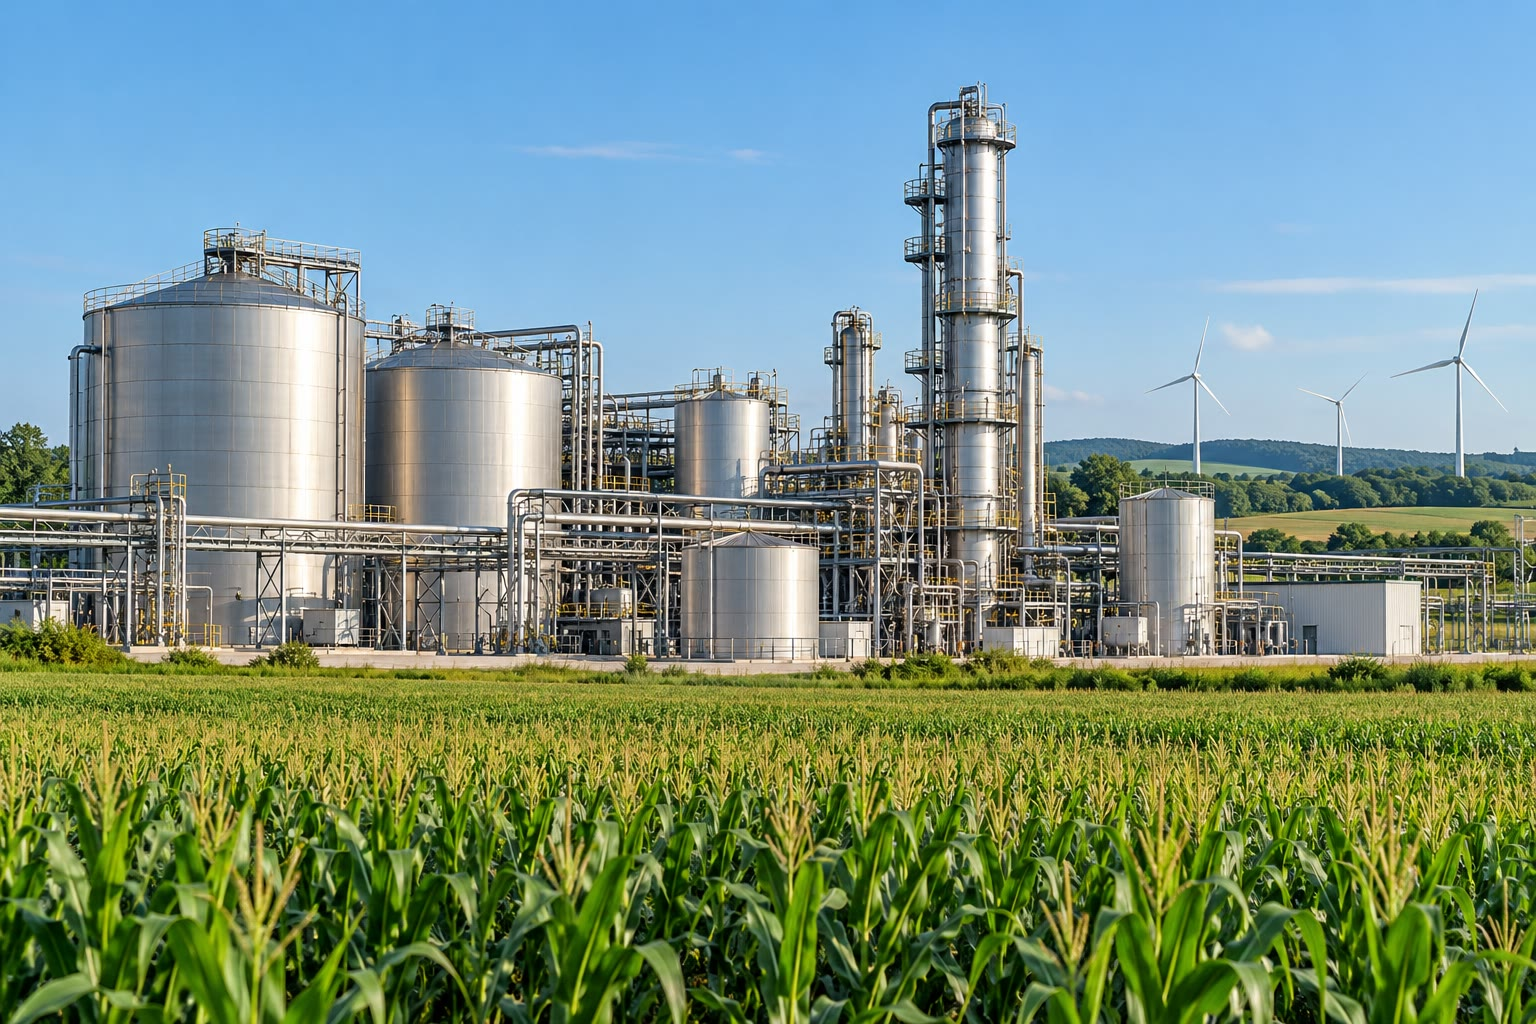
\includegraphics[width=0.58\linewidth]{images/book4/ai/b3-31-biorefinery.jpg}

{\small A biorefinery: fermentation tanks and a distillation column turning
crops and residues into fuels and platform chemicals.}
\end{omfigure}

\section{Measuring greenness}

\begin{definition}[Green chemistry]\label{def:b3:green-industrial:green-chemistry}
\emph{Green chemistry}\index{green chemistry} is the design of chemical
products and processes that reduce or eliminate the use and generation of
hazardous substances, summarised in twelve principles: prevent waste, maximise
\omterm{def:b3:green-industrial:atom-economy}{atom economy}, use and make less hazardous substances, design safer products,
use safer solvents, save energy, use \omterm{def:b3:green-industrial:feedstock}{renewable feedstocks}, avoid unnecessary
derivatives, prefer catalysts to stoichiometric reagents, design for
degradation, monitor in real time, and choose inherently safer chemistry.
\end{definition}

\begin{definition}[Atom economy]\label{def:b3:green-industrial:atom-economy}
The \emph{atom economy}\index{atom economy} of a reaction is the molar mass of
the desired product divided by the sum of the molar masses of all the
reactants in the balanced equation, as a percentage.
\end{definition}

\begin{proposition}[Atom economy by reaction class]\label{prop:b3:green-industrial:ae-classes}
Additions and rearrangements have an \omterm{def:b3:green-industrial:atom-economy}{atom economy} of 100\,\%; substitutions and
eliminations have less.
\end{proposition}

\begin{proof}
In an addition, $\mathrm{A} + \mathrm{B} \to \mathrm{AB}$, or a rearrangement, $\mathrm{A} \to \mathrm{A'}$, the only product contains all the
atoms of the reactants, so its molar mass equals the sum of theirs. A
substitution, $\mathrm{A{-}X} + \mathrm{Y} \to \mathrm{A{-}Y} + \mathrm{X}$, or an elimination, $\mathrm{A} \to \mathrm{B} + \mathrm{C}$, produces a
second product that carries away mass.
\end{proof}

\begin{definition}[E-factor]\label{def:b3:green-industrial:e-factor}
The \emph{E-factor}\index{E-factor} of a process is the mass of waste per mass of
product. In the complete E-factor all inputs not ending in the product count as
waste, solvents and water included; the simple E-factor leaves out solvents and
water.
\end{definition}

\begin{definition}[Process mass intensity]\label{def:b3:green-industrial:pmi}
The \emph{process mass intensity}\index{process mass intensity} (PMI) is the
total mass of materials put into a process (reactants, reagents, solvents,
water) per mass of product.
\end{definition}

\begin{proposition}[PMI and E-factor]\label{prop:b3:green-industrial:pmi-e}
For the same boundary, $\mathrm{PMI} = E + 1$, with $E$ the complete \omterm{def:b3:green-industrial:e-factor}{E-factor}.
\end{proposition}

\begin{proof}
By conservation of mass, everything put in leaves either as product or as waste:
$m_{\mathrm{in}} = m_{\mathrm{product}} + m_{\mathrm{waste}}$. Dividing by $m_{\mathrm{product}}$ gives $\mathrm{PMI} = 1 + E$.
\end{proof}

\begin{definition}[Reaction mass efficiency]\label{def:b3:green-industrial:rme}
The \emph{reaction mass efficiency}\index{reaction mass efficiency} (RME) of a
reaction is the mass of product obtained divided by the total mass of the
reactants used.
\end{definition}

\begin{proposition}[RME from yield and atom economy]\label{prop:b3:green-industrial:rme}
$\mathrm{RME} = \mathrm{AE} \times \text{yield}/\mathrm{SF}$, where the stoichiometric factor $\mathrm{SF} \ge 1$ is the mass of
reactants used divided by the mass the balanced equation requires.
\end{proposition}

\begin{proof}
For one mole of product expected, the equation needs a mass $\sum M_r$ of reactants and
the run uses $\mathrm{SF}\sum M_r$; it gives $\text{yield} \times M_{\mathrm p}$ of product. Dividing:
$\mathrm{RME} = \text{yield}\,M_{\mathrm p}/(\mathrm{SF}\sum M_r) = \mathrm{AE} \times \text{yield}/\mathrm{SF}$.
\end{proof}

\begin{method}[Computing the metrics of a route]\label{met:b3:green-industrial:metrics}
\begin{enumerate}
  \item Write the balanced equation of each step and compute the \omterm{def:b3:green-industrial:atom-economy}{atom economy} of the
        route from all the reactants that enter it.
  \item From the batch record, add the masses of everything charged (reactants,
        reagents, solvents, water, work-up materials): PMI = total in / product.
  \item $E = \mathrm{PMI} - 1$; subtract recovered and reused streams if they are inside the
        boundary, and say so.
  \item RME for each step: product / reactants, to find where material is lost
        (low yield, excess reagent, or poor \omterm{def:b3:green-industrial:atom-economy}{atom economy}).
\end{enumerate}
\end{method}

\begin{omfigure}
\begin{tikzpicture}
\begin{axis}[name=a, width=0.48\linewidth, height=5.4cm, ybar, bar width=14pt, ymin=0, ymax=110,
  xtick={1,2,3,4}, xticklabels={{ibuprofen, 6 steps}, {ibuprofen, 3 steps}, {EO, chlorohydrin}, {EO, direct}},
  x tick label style={font=\scriptsize, rotate=25, anchor=north east}, ylabel={atom economy / \%},
  axis lines=left, tick label style={font=\scriptsize}, label style={font=\small},
  nodes near coords, nodes near coords style={font=\scriptsize, /pgf/number format/fixed, /pgf/number format/precision=0},
  enlarge x limits=0.18]
\addplot[fill=omMeth!55, draw=omMeth] table[x=i, y=AE] {figdata/out/bachelor-3-green-metrics.dat};
\end{axis}
\begin{axis}[at={(a.east)}, anchor=west, xshift=1.4cm, width=0.48\linewidth, height=5.4cm, ybar, bar width=14pt, ymin=0, ymax=3.4,
  xtick={1,2,3,4}, xticklabels={{ibuprofen, 6 steps}, {ibuprofen, 3 steps}, {EO, chlorohydrin}, {EO, direct}},
  x tick label style={font=\scriptsize, rotate=25, anchor=north east}, ylabel={minimum E-factor},
  axis lines=left, tick label style={font=\scriptsize}, label style={font=\small},
  nodes near coords, nodes near coords style={font=\scriptsize, /pgf/number format/fixed, /pgf/number format/precision=2},
  enlarge x limits=0.18]
\addplot[fill=omThm!45, draw=omThm] table[x=i, y=Emin] {figdata/out/bachelor-3-green-metrics.dat};
\end{axis}
\end{tikzpicture}

{\small Atom economies of two routes to ibuprofen and two routes to ethylene oxide
(EO), and the smallest \omterm{def:b3:green-industrial:e-factor}{E-factors} they allow (all yields 100\,\%, no solvent):
$E_{\min} = (1 - \mathrm{AE})/\mathrm{AE}$. Real \omterm{def:b3:green-industrial:e-factor}{E-factors}, with yields below 100\,\%, excess reagents and
solvents, are larger.}
\end{omfigure}

\section{Solvents and energy}

Solvents are usually the largest part of the mass of a fine-chemical or
pharmaceutical process. Solvent selection guides rank them by safety, health and
environmental criteria: water, ethanol, ethyl acetate, 2-methyltetrahydrofuran
and anisole are recommended; dichloromethane, chloroform, benzene, hexane,
dimethylformamide and 1,4-dioxane are to be avoided or banned. Water,
supercritical carbon dioxide (which dissolves non-polar compounds and leaves no
residue when the pressure is released) and solvent-free reactions remove the
problem at its source.

\begin{method}[Using a solvent selection guide]\label{met:b3:green-industrial:solvent-choice}
\begin{enumerate}
  \item List what the solvent must do: dissolve the reactants, survive the reagents,
        boil at a usable temperature, separate from water in the work-up.
  \item Pick from the recommended class first; check its hazard statements.
  \item If a problematic solvent is needed, look for a recommended one with the same
        function (2-methyltetrahydrofuran for dichloromethane or THF in
        extractions, ethyl acetate and heptane for hexane in chromatography).
  \item Plan its recovery by distillation, and count what is lost in the \omterm{def:b3:green-industrial:e-factor}{E-factor}.
\end{enumerate}
\end{method}

\begin{definition}[Process intensification]\label{def:b3:green-industrial:intensification}
\emph{Process intensification}\index{process intensification} is the
redesign of equipment and operating conditions to make a process much smaller,
safer or more efficient: continuous flow reactors with small volumes and
large heat-exchange areas, reactive distillation, microwave heating.
\end{definition}

In a flow reactor only a small volume of a hazardous intermediate exists at any
moment, and heat is removed far faster than in a large batch vessel; reactions
that would run away in a tank can be run at higher temperatures and
concentrations. Catalysts replace stoichiometric reagents, saving both the
reagent and the waste it becomes: the Friedel--Crafts acylation of the old
ibuprofen route used aluminium chloride in stoichiometric amount, destroyed in
the work-up; the new one uses hydrogen fluoride as catalyst and solvent,
recovered and reused.

\section{Life-cycle thinking}

\begin{definition}[Life-cycle assessment]\label{def:b3:green-industrial:lca}
A \emph{life-cycle assessment}\index{life-cycle assessment} (LCA) evaluates the
environmental impacts of a product over its life, from raw-material extraction
to disposal. It is expressed per \emph{functional unit}\index{functional unit},
the service delivered (for example, one wash of a load of laundry), within a
\emph{system boundary}\index{system boundary} that states which processes are
included. A \emph{cradle-to-gate assessment}\index{cradle-to-gate assessment}
stops when the product leaves the factory.
\end{definition}

\begin{omfigure}
\begin{tikzpicture}[font=\scriptsize, >=Stealth,
  box/.style={draw, rounded corners, fill=omDef!10, align=center, minimum height=8mm, inner sep=3pt}]
  \node[box] (r) at (0,0) {raw materials\\ extraction};
  \node[box] (p) at (2.6,0) {chemical\\ production};
  \node[box] (f) at (5.2,0) {formulation,\\ packaging};
  \node[box] (u) at (7.8,0) {use};
  \node[box] (e) at (10.2,0) {end of life:\\ recycling, disposal};
  \foreach \a/\b in {r/p, p/f, f/u, u/e} \draw[->, thick] (\a) -- (\b);
  \draw[omThm, thick, dashed, rounded corners] (-1.1,-0.75) rectangle (3.75,0.75);
  \node[omThm, anchor=north] at (1.3,-0.8) {cradle-to-gate boundary};
  \draw[omMeth, thick, dashed, rounded corners] (-1.25,-1.35) rectangle (11.5,0.95);
  \node[omMeth, anchor=north] at (5.1,-1.4) {cradle-to-grave boundary};
  \node[anchor=south] at (5.1,1.0) {inputs: materials, energy, water \quad outputs: product, emissions, waste};
\end{tikzpicture}

{\small Stages of a product's life and two system boundaries. Inputs and outputs
are inventoried for every process inside the boundary and converted into impact
categories (climate change, acidification, water use, toxicity\dots) per
\omterm{def:b3:green-industrial:lca}{functional unit}.}
\end{omfigure}

\begin{definition}[Carbon footprint]\label{def:b3:green-industrial:carbon-footprint}
The \emph{carbon footprint}\index{carbon footprint} of a product is its
life-cycle emission of greenhouse gases, expressed as the mass of carbon dioxide
with the same warming effect.
\end{definition}

\begin{method}[Setting up a comparative LCA]\label{met:b3:green-industrial:lca}
\begin{enumerate}
  \item State the goal and the \omterm{def:b3:green-industrial:lca}{functional unit}: compare what delivers the same
        service, not the same mass.
  \item Draw the same \omterm{def:b3:green-industrial:lca}{system boundary} for both options.
  \item Inventory inputs and outputs of every process inside it, with data
        sources and dates.
  \item Convert to impact categories, then look for trade-offs (lower carbon but
        more water) and test how sensitive the conclusion is to the data.
\end{enumerate}
\end{method}

\section{Major processes and their improvement}

\begin{proposition}[Carbon dioxide from ammonia]\label{prop:b3:green-industrial:smr}
Making ammonia with hydrogen from steam reforming of methane releases, from the
feedstock alone, $3/8$ mole of $\ce{CO2}$ per mole of $\ce{NH3}$: about \qty{0.97}{t} of $\ce{CO2}$ per tonne of ammonia.
\end{proposition}

\begin{proof}
Reforming followed by the water--gas shift is overall $\ce{CH4 + 2H2O -> CO2 + 4H2}$. The synthesis
is $\ce{N2 + 3H2 -> 2NH3}$: two moles of ammonia need three of hydrogen, that is $3/4$ mole of
methane and $3/4$ mole of $\ce{CO2}$; per mole of ammonia, $3/8$. A tonne of ammonia
(\qty{17.0}{g/mol}) is $\qty{5.88e4}{mol}$, giving $\qty{2.21e4}{mol} \times \qty{44.0}{g/mol} = \qty{0.97}{t}$ of $\ce{CO2}$. Burning methane
for the heat of reforming adds more.
\end{proof}

% ledger: nh3:world-2024
Ammonia plants, which make about 150 million tonnes of nitrogen a year, are among
the largest single sources of industrial carbon dioxide; hydrogen from
electrolysis with low-carbon electricity, or carbon capture at the reformer,
are the routes to cut it. The ammonia loop itself, with its low single-pass
conversion, recycle of unreacted gas and purge of the argon and methane that
would otherwise accumulate, is already efficient.

\begin{omfigure}
\begin{tikzpicture}[font=\scriptsize, >=Stealth,
  box/.style={draw, rounded corners, fill=omMeth!10, align=center, minimum height=8mm, inner sep=3pt}]
  \node[box] (m) at (0,0) {mixer};
  \node[box] (c) at (2.6,0) {compressor};
  \node[box] (r) at (5.2,0) {converter\\ (iron catalyst)};
  \node[box] (s) at (8.0,0) {condenser,\\ separator};
  \draw[->, thick] (-1.8,0) -- (m) node[pos=0, left, align=right] {$\ce{N2 + 3H2}$\\ (make-up)};
  \draw[->, thick] (m) -- (c); \draw[->, thick] (c) -- (r); \draw[->, thick] (r) -- (s);
  \draw[->, thick] (s) -- ++(0,-1.2) node[below] {liquid $\ce{NH3}$};
  \draw[->, thick] (s.north) -- ++(0,0.8) -| node[pos=0.25, above] {recycle of unreacted gas} (m.north);
  \draw[->, thick, omThm] ($(s.north)+(0,0.8)$) -- ++(1.6,0) node[right] {purge (Ar, $\ce{CH4}$)};
\end{tikzpicture}

{\small The ammonia synthesis loop: fresh gas is mixed with recycled gas,
compressed and passed over the catalyst; ammonia is condensed out, the unreacted
gas returns, and a small purge stream removes the inert gases that would
otherwise build up.}
\end{omfigure}

Other large processes show the same lessons. The contact process for sulfuric
acid is so exothermic that a modern plant exports steam and electricity.
Ethylene oxide was first made through ethylene chlorohydrin, with calcium
chloride as waste; direct oxidation of ethylene with oxygen over silver, an
addition with 100\,\% \omterm{def:b3:green-industrial:atom-economy}{atom economy}, replaced it, at the cost of some ethylene burnt to
carbon dioxide. Propylene oxide is now also made with hydrogen peroxide on a
titanium \omterm{def:b3:inorganic-materials:zeolite}{zeolite} catalyst, with water as the only by-product. Adipic acid,
made by oxidising cyclohexanol and cyclohexanone with nitric acid, releases
nitrous oxide, a strong greenhouse gas, which plants now destroy catalytically.

\section{Renewable feedstocks and biocatalysis}

\begin{definition}[Renewable feedstocks]\label{def:b3:green-industrial:feedstock}
A \emph{renewable feedstock}\index{renewable feedstock} is a raw material
replenished on a human time scale, such as plant biomass. A \emph{platform
molecule}\index{platform molecule} is a simple compound made from it in large
amounts and converted into many products: ethanol, lactic acid, succinic acid,
glycerol, levulinic acid, furfural, 5-(hydroxymethyl)furfural.
\end{definition}

\begin{definition}[Biocatalysis]\label{def:b3:green-industrial:biocatalysis}
\emph{Biocatalysis}\index{biocatalysis} is the use of \omterm{def:b3:complex-kinetics:enzyme}{enzymes}, isolated or in
cells, as catalysts for chemical transformations.
\end{definition}

\omterm{def:b3:complex-kinetics:enzyme}{Enzymes} work in water near room temperature with exquisite selectivity, and
directed evolution now tailors them to non-natural substrates: a transaminase
evolved for the purpose replaced a rhodium-catalysed asymmetric hydrogenation
in the manufacture of the diabetes drug sitagliptin, and ketoreductases make many
chiral alcohols. Carbon dioxide itself is a feedstock: urea is made from it and
ammonia, and methanol from it and hydrogen. Polyethylene terephthalate can be
depolymerised by glycolysis or methanolysis back to its monomers, or by
engineered \omterm{def:b3:complex-kinetics:enzyme}{enzymes}, and repolymerised.

\begin{inthelab}[Replacing dichloromethane in a work-up]
A product that was extracted from water with dichloromethane is extracted
instead with 2-methyltetrahydrofuran: it is made from biomass, separates
cleanly from water (it is only partly miscible), and is the upper layer, not
the lower one, which changes the order of the separating-funnel operations. The
organic layers are dried, the solvent distilled off at reduced pressure and
collected for reuse.
\end{inthelab}

\begin{safety}{\ghs[0.62cm]{GHS02}\ghs[0.62cm]{GHS04}\ghs[0.62cm]{GHS06}\ghs[0.62cm]{GHS08}}
% ledger: ghs4:EO, ghs:CH2Cl2, ghs4:2MeTHF
Ethylene oxide: extremely flammable gas under pressure, toxic if inhaled, may
cause cancer and genetic defects; it exists only in closed industrial systems
and sterilisation units. Dichloromethane is a suspected carcinogen, and
2-methyltetrahydrofuran is flammable and corrosive to the eyes: a greener solvent
is not a harmless one.
\end{safety}

\begin{history}[Twelve principles and one number]
Paul Anastas and John Warner published the twelve principles of \omterm{def:b3:green-industrial:green-chemistry}{green
chemistry} in 1998. Roger Sheldon introduced the \omterm{def:b3:green-industrial:e-factor}{E-factor} in 1992, observing that
the fine-chemical and pharmaceutical industries, though small in tonnage,
produced far more waste per kilogram of product than bulk chemistry. The
three-step ibuprofen process, started in 1992, became one of the early
examples of the new approach.
\end{history}

\section{Exercises}

\begin{exercise}[$\star$]\label{exo:b3:green-industrial:1}
Compute the \omterm{def:b3:green-industrial:atom-economy}{atom economy} of the Diels--Alder reaction of butadiene with ethene, of
the esterification of acetic acid with ethanol, and of the Wittig reaction of
benzaldehyde with $\ce{Ph3P=CH2}$ (giving styrene and triphenylphosphine oxide).
\end{exercise}

\begin{exercise}[$\star$]\label{exo:b3:green-industrial:2}
A batch uses 120 kg of materials (reactants, solvents and water) and gives 8.0 kg of
product. Compute PMI and the complete \omterm{def:b3:green-industrial:e-factor}{E-factor}.
\end{exercise}

\begin{exercise}[$\star$]\label{exo:b3:green-industrial:3}
Choose a \omterm{def:b3:green-industrial:lca}{functional unit} for comparing two laundry detergents, and say why
``one kilogram of powder'' would be a poor choice.
\end{exercise}

\begin{exercise}[$\star$]\label{exo:b3:green-industrial:4}
Suggest greener replacements for dichloromethane in an extraction, hexane in
chromatography, and DMF in an amide coupling.
\end{exercise}

\begin{exercise}[$\star\star$]\label{exo:b3:green-industrial:5}
An esterification of 60.0 g of acetic acid with 92.0 g of ethanol (twice the
stoichiometric amount) gives 70.4 g of ethyl acetate. Compute the yield, the \omterm{def:b3:green-industrial:atom-economy}{atom
economy}, the stoichiometric factor and the RME, and check the relation between
them.
\end{exercise}

\begin{exercise}[$\star\star$]\label{exo:b3:green-industrial:6}
Compute the atom economies of the chlorohydrin and direct-oxidation routes to
ethylene oxide, and the mass of calcium chloride made per tonne of ethylene oxide
by the first.
\end{exercise}

\begin{exercise}[$\star\star$]\label{exo:b3:green-industrial:7}
Check the $\ce{CO2}$ per tonne of ammonia of the chapter, and compute the $\ce{CO2}$ per tonne of
hydrogen made by steam reforming.
\end{exercise}

\begin{exercise}[$\star\star$]\label{exo:b3:green-industrial:8}
Compute the minimum electrical energy, in kWh, to make one kilogram of hydrogen by
electrolysis of liquid water at \qty{25}{\celsius}, from $\Delta_rG^\circ$, and the energy from $\Delta_rH^\circ$.
\end{exercise}

\begin{exercise}[$\star\star$]\label{exo:b3:green-industrial:9}
If one mole of $\ce{N2O}$ is formed per mole of adipic acid ($\ce{C6H10O4}$) and the global warming
potential of $\ce{N2O}$ is 273 (data of the exercise), compute the $\ce{N2O}$ and the $\ce{CO2}$ equivalent
per tonne of adipic acid without abatement.
\end{exercise}

\begin{exercise}[$\star\star\star$]\label{exo:b3:green-industrial:10}
Show that for a sequence of steps the overall RME is not the product of the step
RMEs when excess reagents are recycled, and explain how recycling changes the
\omterm{def:b3:green-industrial:e-factor}{E-factor}.
\end{exercise}

\begin{exercise}[$\star\star\star$]\label{exo:b3:green-industrial:11}
A process improvement cuts the solvent in a step from 20 L to 5 L per kilogram of
product (solvent density \qty{0.80}{kg/L}, 90\,\% recovered by distillation before and after; data
of the exercise). Compute the change in the complete \omterm{def:b3:green-industrial:e-factor}{E-factor}.
\end{exercise}

\begin{exercise}[$\star\star\star$]\label{exo:b3:green-industrial:12}
A bio-based route to a monomer has a lower \omterm{def:b3:green-industrial:carbon-footprint}{carbon footprint} but needs more land
and water than the petrochemical route. How would a comparative LCA present this,
and what would you need to decide between them?
\end{exercise}

\section{Problem: Ibuprofen, Six Steps or Three?}

\begin{problem}[{Weekend problem --- ibuprofen, six steps or three: the atom
economies of the two routes, their E-factors, the catalysts that make the
difference, and the waste avoided in a year}]
\label{pb:b3:green-industrial:1}
% ledger: aw:C, aw:H, aw:O, aw:Cl, aw:Na, aw:N
Data of the problem, per tonne of ibuprofen. Three-step route: 0.71 t of
isobutylbenzene, 0.55 t of acetic anhydride, 0.010 t of hydrogen, 0.14 t of carbon
monoxide, 0.05 t of solvent and catalyst losses; 0.31 t of acetic acid recovered
and sold. Six-step route: 2.0 t of reagents and 1.5 t of unrecovered solvents
and auxiliaries. A plant makes 3000 t of ibuprofen a year.

\medskip\noindent\textbf{Part I --- \omterm{def:b3:green-industrial:atom-economy}{Atom economy}.}
\begin{enumerate}
  \item Write the three steps of the catalytic route.
  \item Write its overall equation.
  \item Compute the molar masses involved and the \omterm{def:b3:green-industrial:atom-economy}{atom economy}.
  \item List the reactants of the six-step route (Friedel--Crafts acylation, Darzens
        condensation with ethyl chloroacetate and sodium ethoxide, hydrolysis and
        decarboxylation, oxime formation, dehydration to the nitrile, hydrolysis).
  \item Compute its \omterm{def:b3:green-industrial:atom-economy}{atom economy} from the sum of their molar masses (with two
        waters).
  \item Which by-products leave the old route?
\end{enumerate}

\medskip\noindent\textbf{Part II --- \omterm{def:b3:green-industrial:e-factor}{E-factors}.}
\begin{enumerate}[resume]
  \item Compute the mass put into the new route per tonne of product.
  \item Compute its PMI and its complete \omterm{def:b3:green-industrial:e-factor}{E-factor}, acetic acid counted as waste.
  \item Compute the \omterm{def:b3:green-industrial:e-factor}{E-factor} if the recovered acetic acid is counted as a product.
  \item Compute PMI and \omterm{def:b3:green-industrial:e-factor}{E-factor} for the old route.
  \item Why is the real \omterm{def:b3:green-industrial:e-factor}{E-factor} larger than $(1 - \mathrm{AE})/\mathrm{AE}$?
  \item Which of the twelve principles do the differences illustrate?
\end{enumerate}

\medskip\noindent\textbf{Part III --- Catalysts.}
\begin{enumerate}[resume]
  \item What does hydrogen fluoride replace in the acylation, and why does it matter?
  \item What catalyses the hydrogenation of the ketone to the alcohol?
  \item What catalyses the \omterm{def:b3:homogeneous-catalysis:carbonylation}{carbonylation} of the alcohol, and which chapter's chemistry
        is it?
  \item Why is acetic acid a by-product in both routes?
  \item What hazards does the new route bring, and how are they managed?
  \item Why does fewer steps also mean less energy?
\end{enumerate}

\medskip\noindent\textbf{Part IV --- A year.}
\begin{enumerate}[resume]
  \item Compute the waste of the old route for the plant's annual output.
  \item Compute that of the new route (acetic acid sold).
  \item Compute the waste avoided per year.
  \item Is a lower \omterm{def:b3:green-industrial:e-factor}{E-factor} always a lower environmental impact?
  \item What would a \omterm{def:b3:green-industrial:lca}{life-cycle assessment} add?
  \item State the result: the \omterm{def:b3:green-industrial:atom-economy}{atom economy} of the three-step route.
\end{enumerate}
\end{problem}
